
% This LaTeX was auto-generated from MATLAB code.
% To make changes, update the MATLAB code and republish this document.

\documentclass{article}
\usepackage{graphicx}
\usepackage{color}

\sloppy
\definecolor{lightgray}{gray}{0.5}
\setlength{\parindent}{0pt}

\begin{document}

    
    
\subsection*{Contents}

\begin{itemize}
\setlength{\itemsep}{-1ex}
   \item Load images
   \item Quadratic potential
   \item Discontinous-Huber potential
   \item Discontinous potential
\end{itemize}


\subsection*{Load images}

\begin{verbatim}
clc;clear;close all
load('assignmentImageReconstructionPhantom.mat')
initalIm = ifft2(imageKspaceData);
RRMSE(imageNoiseless,initalIm)
\end{verbatim}

        \color{lightgray} \begin{verbatim}
ans =

    0.2612

\end{verbatim} \color{black}
    

\subsection*{Quadratic potential}

\begin{verbatim}
alpha = 0.935;
priorType = 'quad';
gamma = [];

gradientDescentScript; %actual code in this script. Parameters

figure
subplot(2,3,1)
imshow(real(imageNoiseless))
title('noiseless image')

subplot(2,3,2)
imshow(real(initalIm))
title('noisy image')

subplot(2,3,3)
imshow(real(currentIm))
title('reconstructed image')

subplot(2,3,4)
plot(values)
title('objective values')

subplot(2,3,6)
plot(error_rrmse)
title('RRMSE error')
\end{verbatim}

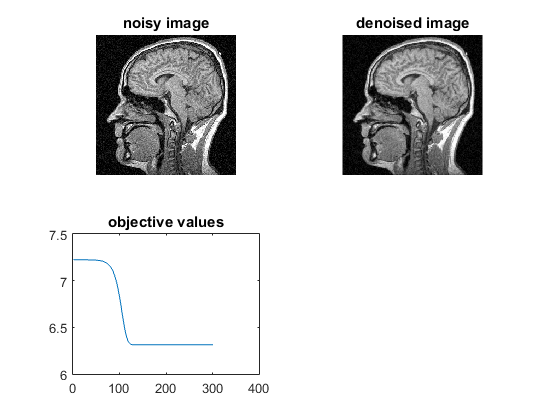
\includegraphics [width=4in]{myDriver_01.eps}


\subsection*{Discontinous-Huber potential}

\begin{verbatim}
alpha = 0.9993;
gamma = 0.005;
priorType = 'disc-huber';

gradientDescentScript;
figure
subplot(2,3,1)
imshow(real(imageNoiseless))
title('noiseless image')

subplot(2,3,2)
imshow(real(initalIm))
title('noisy image')

subplot(2,3,3)
imshow(real(currentIm))
title('reconstructed image')

subplot(2,3,4)
plot(values)
title('objective values')

subplot(2,3,6)
plot(error_rrmse)
title('RRMSE error')
\end{verbatim}

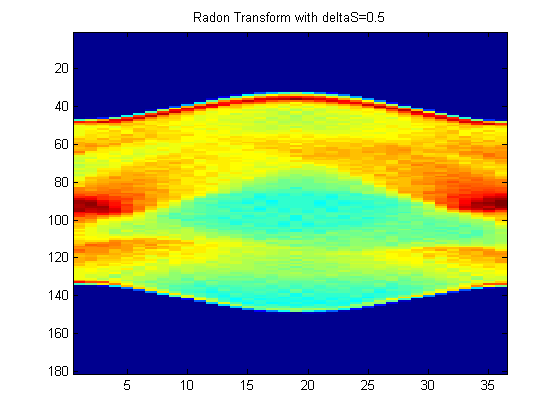
\includegraphics [width=4in]{myDriver_02.eps}


\subsection*{Discontinous potential}

\begin{verbatim}
alpha = 0.99993;
gamma = 0.001;
priorType = 'disc';

gradientDescentScript;

figure
subplot(2,3,1)
imshow(real(imageNoiseless))
title('noiseless image')

subplot(2,3,2)
imshow(real(initalIm))
title('noisy image')

subplot(2,3,3)
imshow(real(currentIm))
title('reconstructed image')

subplot(2,3,4)
plot(values)
title('objective values')

subplot(2,3,6)
plot(error_rrmse)
title('RRMSE error')
\end{verbatim}

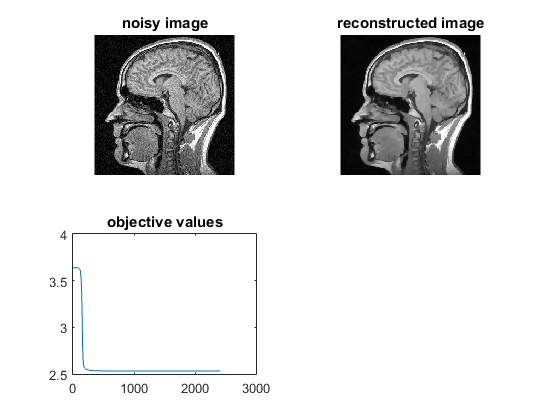
\includegraphics [width=4in]{myDriver_03.eps}



\end{document}
    
